\documentclass{elsarticle}

\usepackage{amsmath}
\usepackage{amsfonts}
\usepackage{amssymb}
\usepackage{stmaryrd}
\usepackage{color}
\usepackage{graphicx}
\usepackage{hyperref}

\newtheorem{prop}{Proposition}

\def\Laplace{\Delta}
\def\prtl{\partial} % partial deriv.
\def\grad{\nabla}
\def\vc#1{\mathbf{\boldsymbol{#1}}}     % vector
\def\todo#1{{TODO:\color{red}#1}}
\def\ol#1{\overline{#1}}
\def\log{{\rm log}}


%opening

% Possible Journals:
% https://agupubs.onlinelibrary.wiley.com/doi/abs/10.1029/WR026i010p02331

\begin{document}

\begin{frontmatter}

\title{Analytical solution to a single fracture test problem
%\thanks{This work was supported by the Technology Agency of the Czech Republic under the project no. TA01021331. }
}
\author[1]{Jan B\v rezina\corref{cor1}%
\ead{jan.brezina@tul.cz}}
\cortext[cor1]{Corresponding author}
\address[1]{Technical University in Liberec, Studentsk\'a 2, Liberec, Czech Republic.}
\author[2]{Pavel Burda%
\ead{pavel.burda@fs.cvut.cz}}
\address[2]{Czech Technical University, Prague, Czech Republic.}

\begin{abstract}
The Fourier method is used to derive an analytical solution to a Darcy flow problem on a square domain with a single discrete fracture. Distinct pressure variables are considered for the fracture and the matrix respectively coupled together by a 
Robin-type condition. 
Two cases are treated: the conductive fracture with pressure continuous and symmetric about the fracture and the barrier fracture,
a generalization with separate pressure and matrix parameters for the upper and the lower part of the domain. The analytical solution is verified against the numerical solution using second-order finite differences. 
\end{abstract}

\begin{keyword}
Darcy flow,
fractured porous media,
analytical solution, 
fourier series
%% keywords here, in the form: keyword \sep keyword

%% PACS codes here, in the form: \PACS code \sep code

%% MSC codes here, in the form: \MSC code \sep code
%% or \MSC[2008] code \sep code (2000 is the default)

\end{keyword}

\end{frontmatter}


%\begin{keywords} 
%fracture flow, mortar methods, mixed-hybrid finite elements
%\end{keywords}

%\begin{AMS}
%15A15, 15A09, 15A23
%\end{AMS}



\section{Introduction}
\todo{Add references for:
fracture flow applications, DFN description vs. Continuum flow description, explain different papaers dealing with C-F approach. 
Reference for classical Fourier method.}

Fractures, cracks, fissures, faults, and other discontinuities are ubiquitous  especially in crystaline rocks.  Although they occupy a tiny fraction of the rock volume their impact
on the groundwater flow is significant. Open fractures and their systems form preferential paths with much larger Darcian velocity. This heterogeneity leads to much smaller breakthrough times in the transport of contaminants. On the other hand, the healed fractures can behave as barriers.
\todo{More general applications, to the fracture flow}


\todo{DEscribe farctal nature of the fracture networks and DFN vs. continuum models vs. CF model}
Fractures occur occur on a wide range of scales. Small scale fractures can be modeled by modified average permeability of the rock, while the large fractures at the scale comparable to the dimensions of a domain should be described explicitly in order to capture preferential paths. Even the large-scale fractures are still very thin and their direct discretization by 3d elements leads to high levels of mesh refinement which become 
costly especially for a large number of fractures. A solution to this problem is the usage of a {\it mixed mesh} combining the elements of a different dimension. It has been shown that for the advection-diffusion equation the original 3d (or 2d) problem can be approximated by the system of 3d-2d (or 2d-1d) problems coupled by a Robin type condition (see e.g. \cite{Martin2005}, \cite{fumagalli_numerical_2011}, \cite{Angot},\cite{brezina_analysis_2015}). 

For the purpose of testing the implementation of various numerical schemes for advection-diffusion equations on the mixed mesh, it is necessary to have a suitable test problem with a known solution. A common approach is to plug any function into the equations and prescribe the resulting right-hand side. This approach is convenient to test the correctness of the implementation but often turns out to
do not capture peculiarities of the real solution and thus may be unsuitable for tests of convergence of the used method. 




To this end, we propose a test Darcy flow problem consisting of the square domain (matrix) and the single horizontal fracture 
cutting the domain into the upper and lower parts.  
Two cases are considered: the {\it conductive fracture} and the more general {\it barrier fracture}.
The conductive fracture assumes symmetry about the fracture yet keeping separate pressure for the matrix and for the fracture. 
This case is relatively simple to solve but has very limited practical usage.
The barrier fracture case is a generalization where the problem parameters, as well as the matrix pressure, are treated independently on
 the upper and the lower part of the matrix domain. Both problems are introduced in Section \ref{sec:setting}.
The solution to the conductive fracture problem is derived in Section \ref{sec:continuous_frac} the same approach with necessary modifications and extensions
is used to derive the solution to the barrier fracture problem in Section \ref{sec:barrier_frac}. In Section \ref{sec:verify}, 
both solutions are verified against a numerical solution provided by the second-order finite difference scheme on a regular grid. 
Conclusions are summarized in the final Section \ref{sec:conclusion} 


Book about Fourier method:
\cite{Brown1993}

Application of the Furier method to the Darcy flow problems: \cite{Onder1998}


\section{Test problems}
\label{sec:setting}
The main result of the paper is the derivation of the strong analytical solution for two test problems with coupling between continuum and a fracture.
A Darcy flow is considered  on a square 2D domain $\Omega_2 = (-1,1)\times(-1,1)$
with a horizontal fracture $\Omega_1 = { (x,0) : x\in (-1,1)}$. The fracture splits $\Omega_2$ into upper and 
lower part $\Omega_2^+$ and $\Omega_2^-$, respectively.
The stationary Darcy flow is driven by the same equation on all three domains:
\begin{align}
  \label{eq:Darcy_common}
  -k_2 \Laplace p^+_2(x,y) &= 0 \qquad &&\text{ on }\Omega_2^+,\\
  -k_2 \Laplace p^-_2(x,y) &= 0 \qquad &&\text{ on }\Omega_2^-,\\
  -k_1 p_1''(x) &= f(x) \qquad &&\text{ on }\Omega_1.
  \label{eq:Darcy_common_c}
\end{align}
Where $p_d$, $d=1,2$ is the pressure and $f$ is the communication term that will be specified later. 
We consider positive constant conductivities $k_2$, $k_1$ on $\Omega_2$ and $\Omega_1$, respectively.

The homogeneous Neumann condition is set on the left and the right side of $\Omega_2$,
while the Dirichlet condition is set on the top and bottom and at the tips of the fracture.
We denote:
\begin{align*}
   \Gamma^N_2 &= \{(x,y)\, :\, x\in\{-1, 1\},\ y\in (-1, 1),\ y\ne 0\},\\
   \Gamma^N_2 &= \{(x,y)\, :\, x\in (-1, 1),\ y\in \{-1, 1\}\},\\
   \Gamma_1   &= \prtl \Omega_1 = \{(-1, 0),\ (1, 0)\}. 
\end{align*}
Then we prescribe following boundary conditions
\begin{align}
  \label{eq:bc_common}
  \prtl_x p_2(x,y) &= 0  &&\text{ on } \Gamma_2^N\\
  p_2(x,y) &= P_2        &&\text{ on } \Gamma_2^D\\
  p_1(x) &= P_1          &&\text{ on } \Gamma_1.
  \label{eq:bc_1}
\end{align}

To complete the problem, we must prescribe boundary conditions on the fracture and specify the source term $f$. Here we 
distinguish two cases: the \emph{conductive fracture} and the \emph{barrier fracture}.


{\bf Conductive fracture.} In this case, we assume a fracture with similar or higher conductivity than in the continuum, $k_1 \ge k_2$.
In such case, we can assume continuity of the pressure across the fracture. However we keep difference between $p_2$ and $p_1$ on the fracture.
We set:
\begin{align}
  \label{eq:c_coupling_a}
  p_2^+ &= p_2^-                &&\text{ on }\Omega_1,\\
  -k_2 (-\prtl_y p_2^+ + \prtl_y p_2^-) &= f(x)         &&\text{ on }\Omega_1,\\
  f(x) &= 2\sigma (p_2(x,0) - p_1(x)),   &&
  \label{eq:c_coupling_c}
\end{align}
where $\sigma \ge 0$ is a coupling parameter, usually $\sigma \approx k_1 / \delta$ with $\delta$ standing for the fracture cross-section. 
Solution of this case is discussed in Section \ref{sec:continuous_frac}.



{\bf Barrier fracture.} Other case is a fracture with significantly smaller conductivity compared to the surrounding continuum. In this case
the pressure $p_2$ is discontinuous across the fracture and we have two independent boundare conditions for each side of the fracture. We also 
distinguish conductivities $k_2^+$, $k_2^-$ and boundary pressure $P_2^+$, $P_2^-$ for the upper and lower domains $\Omega_2^+$, $\Omega_2^-$, 
respectively. The coupling on the fracture is prescribed by the boundary conditions:
\begin{align}
  \label{eq:bc_barrier_p}  
  - k_2^+ \grad p_2^+\cdot \vc n^+(x,0) &= k_2^+ \prtl_y p_2^+(x) = f^+(x) 
                    &&\text{ on }\Gamma^{+},\\
  \label{eq:bc_barrier_m}
  - k_2^- \grad p_2^-\cdot \vc n^-(x,0) &= -k_2^- \prtl_y p_2^-(x) = f^-(x) 
                    &&\text{ on }\Gamma^{-},
\end{align}
with $\Gamma^{+}$ and $\Gamma^{-}$ denoting boundary of $\Omega_2^+$ and $\Omega_2^-$, respectively, collocated with $\Omega_1$.
The communication term is:
\begin{equation}
  \label{eq:coupling_barrier}
  f(x) = f^+(x) + f^-(x),\quad f^{+/-} = \sigma^{+/-} (p^{+/-}_2(x,0) - p_1(x)),
\end{equation}
where $\sigma^+$ and $\sigma^-$ are positive coupling parameters for uppar and lower side of ther fracture respectively. 
Solution to this system is discussed in Section \ref{sec:barrier_frac}. 

\section{Conductive fracture }
\label{sec:continuous_frac}
We shall derive an analytical solution to the system $(\ref{eq:Darcy_common} - \ref{eq:bc_1})$ with the coupling conditions 
$(\ref{eq:c_coupling_a} - \ref{eq:c_coupling_c})$. Symmetry of the problem in 
both $x$ and $y$ direction allows us to solve equivalent reduced problem on $\widetilde\Omega_2=(0,1)\times(0,1)$ and  
$\widetilde\Omega_1$. We impose the symmetry in $x$ direction by homogeneous Neumann condition at $x=0$. 
All equations are preserved with exception of the half flux on $\Gamma^+$. The equivalent system  reads:
\begin{align}
    \label{eq:cc_darcy_2d}
    -k_2 \Laplace p_2(x,y) &= 0         &&\text{on }\widetilde\Omega_2 \\
    \label{eq:cc_darcy_1d}
    -k_1 p_1''(x) &= f(x)               &&\text{on }\widetilde\Omega_1
\end{align}
with boundary conditions:    

\begin{equation}
    \label{eq:cc_bc_x}
    p_2(x, 1) = P_2, \quad
    k_2\prtl_y p_2(x,0) = \frac{f(x)}{2}
                        = \sigma(p_2(x,0) - p_1(x))
\end{equation}
for  $x\in (0,1)$,
\begin{equation}
    \label{eq:cc_bc_y}
    \prtl_x p_2(0,y) = \prtl_x p_2(1,y) = 0    
\end{equation}
for $y \in (0, 1)$ and finally
\begin{equation}
    \label{eq:cc_bc_1}
    p_1'(0) = 0, \quad  p_1(1) = P_1. 
\end{equation}

%%%%%%%%%%%%%%%%%%%%%%%%%%%%%%%%%%%%%%%%%%% PROPOSITION 1
\begin{prop}
\label{proposition_continuous}
Let the real parameters $P_2$, $P_2$, $k_1>0$, $k_2>0$, $\sigma\ge0$ be given. Then the solution $p_1(x)$ and $p_2(x,y)$ to the system 
$(\ref{eq:cc_darcy_2d} - \ref{eq:cc_bc_1})$ can be expressed in from of Fourier series:
\begin{equation}
    \label{eq:p2_series}
    p_2(x,y) = P_2 + B_0(y-1) -2B_0 \sum_{n=1}^\infty a_n \cos(\pi n x) {\rm sinh} \big(\pi n(1-y)\big)  \ \ ,
\end{equation}
%
\begin{equation}
    \label{eq:p1_series}
    p_1(x) = P_2-B_0 +u_0 \cosh(x/k) -2B_0 \sum_{n=1}^\infty  u_n \cos(\pi n x) 
\end{equation}

where we denote:
\[
    k = \sqrt{\frac{k_1}{2\sigma}}, 
\]    
and use following coefficients:

\begin{equation}
    \label{eq:an}
    a_n = \frac{(-1)^n k_2}{ k_2 \pi n \cosh(\pi n) \big(1 + (k n \pi)^2\big) 
    + \sigma (k n \pi)^2 \sinh(\pi n)} \ , 
\end{equation}

\begin{equation}
    \label{eq:u0}
    u_0 = -\frac{k_2 B_0}{\sigma k\sinh(1/k)}.
\end{equation}

\begin{equation}
    \label{eq:un}
    u_n = \frac{a_n \sinh(n \pi)}{1 + (k n \pi)^2}, 
\end{equation}

and constants:
\begin{equation}
     \label{eq:b0}
     B_0 = \frac{P_2 - P_1}{1 + 2  U + \frac{k_2}{\sigma k} \frac{\cosh(1/k)}{\sinh(1/k)}} 
\end{equation}
\begin{equation}
    \label{eq:U}
    U =  \sum_{n=1}^{\infty} (-1)^n u_n.
\end{equation}

\end{prop}


\subsection{\bf Separation of variables for 2D equation}
\label{sec:p2_conductive}

We shall apply the separation of variables  (see e.g. \cite{Evans1998}) to the equation \eqref{eq:cc_darcy_2d}.  


Considering a solution in form:
\begin{equation}
    \label{eq:sep_vars}
    p_2(x,y) = X(x)Y(y) 
\end{equation}
the equation \eqref{eq:cc_darcy_2d} gives us two equations:
\[
\frac{X''}{X} = -\frac{Y''}{Y} = L\ ,
\]
$L$ being a real constant. Applying homogeneous Neumann boundary conditions \eqref{eq:cc_bc_y}
we get possible solutions $X(x)$ in the form: 
\begin{equation}
    \label{eq:general_x}
    X_n(x) = \tilde A_n + \tilde B_n \cos (n\pi x)\qquad \text{ for }n=0,1, \dots
\end{equation}
where $\tilde A_n$, $\tilde B_n$ are arbitrary real constants and $L$ is quantized to values:
\[
    L= - n^2 \pi^2.
\]


Next we plug $L$ in the equation for $Y(y)$ to get all solutions:
\begin{align}
Y_0(y) &= \tilde C_0 + \tilde D_0 y, \nonumber \\
\label{eq:general_y}
Y_n(y) &= \tilde C_n e^{n\pi y}+ \tilde D_n e^{-n\pi y}\qquad \text{ for } n =1, \dots
\end{align}
where $\tilde A_n, \tilde B_n$ for $n=0,1,\dots$ are arbitrary real constants.

Combining \eqref{eq:sep_vars}, \eqref{eq:general_x}, \eqref{eq:general_y} we can write the solution $p_2$ as:
\begin{equation}
    \label{eq:p2_1}
    p_2(x, y) = A_0 + B_0 y + \sum ^{\infty}_{n=1} \big(C_n + \cos (n\pi x)\big) 
            \frac{1}{2}\big(A_n e^{n\pi (y-1)} + B_n e^{-n\pi (y-1)}\big).
\end{equation}
Then the Dirichlet condition $(\ref{eq:cc_bc_x}a)$ yields:
\[
    P_2 = A_0 + B_0 + \sum ^{\infty}_{n=1} \big(C_n + \cos (n\pi x)\big) 
            \frac{A_n  + B_n}{2}.
\]
for all $x\in (0, 1)$ and thus:
\[
    A_0 + B_0 = P_2, \quad\text{ and } \quad A_n+B_n = 0.
\]
Then \eqref{eq:p2_1} can be simplified to the final form \eqref{eq:p2_series} where we yet have to determine $B_0$ and coefficients $a_n$.


\subsection{Pressure on fracture}
\label{sec:p1_conductive}

 Next step is a solution to the equation on fracture, i.e. \eqref{eq:cc_darcy_1d}. 
 Substituting for $f$ using $(\ref{eq:cc_bc_x})$ and then for $p_2$ from \eqref{eq:p2_series}
 we arrive at: 
\begin{equation}
    \label{eq:p1_equation}
    -k^2 p_1''(x) + p_1 (x) = P_2 - B_0 - 2 B_0 \sum ^{\infty}_{n=1} a_n \sinh(n\pi)\, \cos (n\pi x).
\end{equation}
with $k = \sqrt{k_1 / (2 \sigma)}$.

Solution to:
\[
    - a P''(x) + P(x) = \cos(n \pi x) 
\]    
is 
\[
    P(x) = \frac{\cos(n \pi x)}{1+an^2\pi^2}.
\]
Using linearity of the equation we obtain the general form of $p_1$ as:
\begin {equation}
    \label{eq:p1_general_sol}        
    p_1(x) = c^+ e^{x/k} + c^- e^{-x/k} + P_2 - B_0 
    - 2 B_0 \sum^{\infty}_{n=1} u_n \cos (n\pi x).
\end {equation}
with $u_n$ given by \eqref{eq:un}. Then the boundary conditions \eqref{eq:cc_bc_1} yield:
\begin{align*}
P_1 &= p_1(1) = c^+e^{1/k} + c^- e^{-1/k} + P_2 - B_0 - 2 B_0 U, \\
0 &= p_1'(0) = \frac{1}{k}(c^+ - c^-) 
\end{align*}
with $U$ given by \eqref{eq:U}. Solving for $c^+$ and $c^-$ we get:
\[
  c^+ = c^- = \frac{P_1 - P_2 + B_0(1 + 2 U)}{2\cosh(1/k)}.
\]
Then \eqref{eq:p1_general_sol} gives 
\begin{equation}
    \label{eq:p1_series_tmp}
    p_1(x) = P_2 -  B_0 + u_0 \cosh(x/k) - 2B_0 \sum_{n=1}^\infty  u_n \cos(\pi n x) 
\end{equation}
which is \eqref{eq:p1_series} but with 
\begin{equation}
    \label{eq:u0_def}    
    u_0 = \frac{P_1 - P_2 + B_0 + 2 B_0 U}{\cosh(1/k)}.
\end{equation}



\subsection{Fracture coupling}
\label{sec:cont_coupling}

Last relation that we have to consider is the boundary condition $(\ref{eq:cc_bc_x}b)$. To this end we plug in the relations \eqref{eq:p2_series}, 
\eqref{eq:p1_series_tmp} for $p_2$, $p_1$  and we group the terms for remaining unknowns on the left hand side. After straight forward
manipulation we obtain:
%  \[
%      \frac{B_0 k_2}{\sigma} + 2 B_0 \sum_{n=1}^\infty 
%          \Big[ \frac{k_2}{\sigma} n\pi  \cosh(\pi n) 
%          + \sinh(\pi n)
%          - \frac{\sinh(n \pi)}{1 + (k n \pi)^2} 
%          \Big] a_n
%          \cos(\pi n x)        
%         = - u_0 \cosh(x/k) 
%  \]



\begin{equation}
    \label{eq:conductive_fourier_coupling}
    \frac{{\cal A}_0}{2} + \sum^{\infty}_{n=1} {\cal A}_n \cos (n\pi x) =  - u_0 \cosh(x/k).
\end{equation}
with
\begin{equation}
    \label{eq:fourier_A0}
    {\cal A}_0 = \frac{2 k_2 B_0}{\sigma} 
\end{equation}


\begin{equation}
    \label{eq:fourier_An} 
        {\cal A}_n = 2B_0 \Bigl[ \frac{k_2}{\sigma} n\pi \cosh(n\pi) - \frac{\sinh(n \pi)}{1 + (k n \pi)^2}  
    + \sinh(n \pi) \Bigr]a_n
\end{equation}

for $n=1, \dots$. The left hand side of \eqref{eq:conductive_fourier_coupling} is the Fourier series, thus we determine
remaining unknowns $B_0$, $A_n$ by computing Fourier of the function on the right hand side and comparing coefficients.

For the zero term we have:
\begin{equation}
    \label{eq:compute_A0}
    {\cal A}_0 = -2 u_0 \int _0^1 \cosh(x/k) dx =
    - 2 u_0 k\sinh(1/k).
\end{equation}

which compared to \eqref{eq:fourier_A0} gives us \eqref{eq:u0}.


For other terms, we integrate by parts to get:
\begin{equation}
    \label{eq:compute_An}
    {\cal A}_n = -2 u_0\int _0^1 \cosh(x/k) \cos (n\pi x) dx 
    = -\frac{(-1)^n 2u_0 k}{1+(k n \pi)^2}\sinh(1/k).
\end{equation}

%\[
% k_2   = \Bigl[ ({1+(k n \pi)^2}) k_2 n\pi \cosh(n\pi) + \sigma(k n \pi)^2\sinh(n \pi) \Bigr]a_n
%\]

We plug \eqref{eq:u0} into the result and compare it with \eqref{eq:fourier_An} to obtain
formula \eqref{eq:an} for coefficients $a_n$.
The only remaining unknown is $B_0$ which we determine by comparing \eqref{eq:u0_def} and \eqref{eq:u0}.
Straight forward calculation leads to \eqref{eq:b0}.

\subsection{Evaluation procedure}
Formulas in Proposition \ref{proposition_continuous} are not suitable for practical calculations since hypergeometric functions are evaluated for large $n$.
To remedy this issue, we factor out and cancel $e^{\pi n}$. Actual evaluation then takes  following procedure:

\begin{enumerate}
    \item Set finite $N$ for truncated series. 
    \item Compute $\tilde a_n$ for $n = 1, \dots, N$ using:
    \[
        \tilde a_n = \frac{(-1)^n k_2}{ k_2 \pi n (1 - e^{-2\pi n}) \big(1 + (k n \pi)^2\big) 
            + \sigma (k n \pi)^2 (1 + e^{-2\pi n})} \ , 
    \]
    \item Compute related $\tilde u_n$ coefficients:
    \[
        \tilde u_n = \frac{\tilde a_n (1 - e^{-2\pi n})}{1 + (k n \pi)^2}, 
    \]
    \item Evaluate truncated sum:
    \[
        U =  \sum_{n=1}^{N} (-1)^n u_n.
    \]
    \item Compute remaining parameters $u_0$, $B_0$ using \eqref{eq:u0}, \eqref{eq:b0}.
    \item Evaluate $p_2$ for any given point $(x,y)$ in $\Omega_2$ by:
    \[
        p_2(x,y) = P_2 + B_0(y-1) -2B_0 \sum_{n=1}^N \tilde a_n \cos(\pi n x) 
        \Big( e^{-\pi n |y|} - e^{\pi n (|y|-2)}\Big).
    \]
    \item Evaluate $p_1$ for any given $x$ in $\Omega_1$ by:
    \[
        p_1(x) = P_2 - B_0 + u_0 \cosh(x/k) - 2 B_0 \sum_{n=1}^N  u_n \cos(\pi n x). 
    \]    
\end{enumerate}

Convergence rates of the sums are reasonable. For $a_n$ we have:
\[
    \tilde a_n \approx (-1)^n n^{-3} 
\]
and for two consecutive terms:
\[
    \tilde a_n + \tilde a_{n+1} \approx n^{-3} - (n+1)^{-3} \approx  n^{-4}. 
\]
Series for $p_2$ converge exponentially for $y\ne 0$. Error for $y=0$ is of order $N^{-3}$ with exception
of  $x=1$ where $\cos(\pi n)$ cancels alternation in $a_n$ and error is $N^{-2}$.

Even better is convergence of $u_n$ sums, since:
\[
    u_n \approx (-1)^n n^{-5},\qquad u_n+u_{n+1} \approx  n^{-6}.
\]
Thus for calculation of $p_1$ we have error  $N^{-5}$ (for $x=1$ only $N^{-4}$). The error of $U$ is only $N^{-4}$ 
as the sign alternation cancels with alternation of $a_n$.
The practical behavior of errors follows these estimates.



\section{Barrier fracture}
\label{sec:barrier_frac}
The case with discontinuous $p_2$ across the fracture is solved by the same approach as the continuous case, 
but the derivation is slightly more technical. Considering the $y$ axis symmetry of the problem $(\ref{eq:Darcy_common} - \ref{eq:bc_1})$ and 
the coupling $(\ref{eq:bc_barrier_p} - \ref{eq:coupling_barrier})$, we can consider the same system of equations 
on reduced domains $\Omega_2^+ = (0,1)\times (0,1)$, $\Omega_2^- = (0,1)\times(-1,0)$,
$\Omega_1 = (0,1)$. To impose the symmetry we consider homogeneous Neumann boundary condition on the $y$ axis $\{(0,y)\}$.

Repeating arguments from Section \ref{sec:p2_conductive} we obtain Fourier expansion for $p_2^+$ and $p_2^-$ similar to \eqref{eq:p2_series}:
\begin{align}
    \label{eq:p2_barrier_p}
    p_2^+(x,  y) &= P_2^+ + B_0^+(y-1) - \ol{u}_0\sum_{n=1}^\infty a_n^+ \cos(\pi n x) {\rm sinh} \big(\pi n(1-y)\big),\\ 
    \label{eq:p2_barrier_m}
    p_2^-(x, -y) &= P_2^- + B_0^-(y-1) - \ol{u}_0\sum_{n=1}^\infty a_n^- \cos(\pi n x) {\rm sinh} \big(\pi n(1-y)\big).
\end{align}
with some variable $\ol{u}_0$ to be specified later.

The equation for $p_1$ on $\Omega_1$ can be converted to the form similar to \eqref{eq:p1_equation}:
\begin{equation}
    \label{eq:p1_barrier_equation}
    - \ol{k}  p_1''(x) + p_1(x) = \ol{P}_2 - \ol{B}_0 - \ol{u}_0\sum_{n=1}^{\infty} \ol{a}_n \cos(n \pi x) \sinh(n \pi)
\end{equation}
where we have used averaged variables:

% \begin{align}
%     \label{eq:avg_sigma}
%     \ol{\sigma} &= (\sigma^+ + \sigma^-), \\
%     \label{eq:avg_k}
%     \ol{k} &= \sqrt{k_1/\ol{\sigma}},\\
%     \label{eq:avg_P2}
%     \ol{P}_2 &= \frac{\sigma^+ P_2^+ + \sigma^- P_2^-}{\ol{\sigma}}, \\
%     \label{eq:avg_B0}
%     \ol{B}_0 &= \frac{\sigma^+ B_0^+ + \sigma^- B_0^-}{\ol{\sigma}}, \\
%     \label{eq:avg_an}
%     \ol{A}_n &= \frac{\sigma^+ A_n^+ + \sigma^- A_n^-}{\ol{\sigma}}.  
% \end{align}

\begin{gather*}
    \ol{\sigma} = (\sigma^+ + \sigma^-), \qquad
    \ol{k} = \sqrt{k_1/\ol{\sigma}}, \qquad
    \ol{P}_2 = \frac{\sigma^+ P_2^+ + \sigma^- P_2^-}{\ol{\sigma}}, \\
%    
    \ol{B}_0 = \frac{\sigma^+ B_0^+ + \sigma^- B_0^-}{\ol{\sigma}}, \qquad
    \ol{a}_n = \frac{\sigma^+ a_n^+ + \sigma^- a_n^-}{\ol{\sigma}}.  
\end{gather*}

Then we can repeat steps from Section \ref{sec:p1_conductive} to get $p_1$ expansion that closely follows
\eqref{eq:p1_series_tmp}:

\begin{equation}
    \label{eq:barrier_p1_series}
    p_1(x) = \ol{P}_2 -  \ol{B}_0 + \ol{u}_0 \cosh(x/\ol{k}) - \ol{u}_0 \sum_{n=1}^\infty  \ol{u}_n \cos(\pi n x) 
\end{equation}
where we finally identify $\ol{u}_0$ as:
\begin{equation}
    \label{eq:barrier_u0_def}    
    \ol{u}_0 = \frac{P_1 - \ol{P}_2 + \ol{B}_0 - \ol{u}_0 \ol{U}}{\cosh(1/\ol{k})},
\end{equation}
and we set:
\begin{equation}
    \label{eq:barrier_un}
    \ol{u}_n = \frac{\ol{a}_n \sinh(n \pi)}{1 + (\ol{k} n \pi)^2}, \qquad
    \ol{U} =  -\sum_{n=1}^{\infty} (-1)^n \ol{u}_n.
\end{equation}

\subsection{Coupling}

As in Section \ref{sec:cont_coupling}, we plug expansion of $p_2^+$, $p_2^-$, and $p_1$ into \eqref{eq:bc_barrier_p} and \eqref{eq:bc_barrier_m}. 
We group the terms to get Fourier expansion on the left hand side and a known function of $x$ on the right hand side.
In particular on  $\Gamma^+$ we have:
% \[
%   \frac{k_2^+ B_0^+}{\sigma^+} - P_2^+ + \ol{P}_2) + B_0^+ - \ol{B}_0
%   +\sum_{n=1}^{\infty} \Big[
%         2 \frac{k_2^+ B_0^+}{\sigma^+}  a_n^+ ( n \pi)  \cosh(n \pi) 
%        + 2B_0^+  a_n^+  \sinh(\pi n)   
%        -2\ol{B}_0 u_n   
%         \Big]
%         \cos(n \pi x)  
%   = 
%    - u_0 \cosh(x/\ol{k})
% \]
% 

\begin{equation}
    %\label{eq:fourier_coupling}
    \frac{{\cal A}_0^+}{2} + \sum^{\infty}_{n=1} {\cal A}_n^+ \cos (n\pi x) =  - \ol{u}_0 \cosh(x/ \ol{k}).
\end{equation}
with
\begin{align}
    \label{eq:calA0_1}
    \frac{{\cal A}_0^+}{2} &= \frac{k_2^+ B_0^+}{\sigma^+} - P_2^+ + \ol{P}_2 + B_0^+ - \ol{B}_0\\
    \label{eq:calAn_1}
    {\cal A}_n^+          &=  \ol{u}_0 a_n^+ \Big( n \pi \frac{k_2^+ }{\sigma^+}  \cosh(n \pi) 
        +     \sinh(\pi n)  \Big) 
        - \ol{u}_0 \ol{u}_n   
\end{align}
We reuse the calculation of Fourier coefficients of the right hand side from \eqref{eq:compute_A0} and \eqref{eq:compute_An} to obtain:
\begin{align}
    \label{eq:calA0_2}
    {\cal A}_0^+ &= - 2 \ol{u}_0 \ol{k}\sinh( 1/\ol{k} ), \\
    \label{eq:calAn_2}
    {\cal A}_n^+ &=  - \frac{(-1)^n  2 \ol{u}_0 \ol{k}}{1+(\ol{k} n \pi)^2}\sinh(1/\ol{k}).
\end{align}
Analogous relations hold for the lower side on $\Gamma^-$.

Now we combine \eqref{eq:calAn_1} and \eqref{eq:calAn_2}, we cancel $\ol{u}_0$, and we substitute for $\ol{u}_n$ using \eqref{eq:barrier_un}.
Performing the same operation for the ${\cal A}_n^-$  we obtain a system to determine $a_n^+$, $a_n^-$:

\begin{equation}
    \label{eq:an_system}
    \begin{pmatrix} 
            X_n^{00} & X_n^{01} \\ 
            X_n^{01} & X_n^{11}
    \end{pmatrix}
    \begin{pmatrix} 
        a_n^+  \\ 
        a_n^-     
    \end{pmatrix}
     =  
    \begin{pmatrix} 
        \sigma^{+}y_n \\ 
        \sigma^{-}y_n
    \end{pmatrix}
\end{equation}
where
% \[
% -\frac{2u_0 \ol{k}}{1+(\ol{k} n \pi)^2}\sinh(1/\ol{k}) = A_n^+ \Big( n \pi \frac{k_2^+ }{\sigma^+}  \cosh(n \pi) 
%         +     \sinh(\pi n)  \Big) 
%         - \frac{\sigma^+ A_n^+}{\ol{\sigma}}\frac{\sinh(n \pi)}{1 + (\ol{k} n \pi)^2}
%         - \frac{\sigma^- A_n^-}{\ol{\sigma}}\frac{\sinh(n \pi)}{1 + (\ol{k} n \pi)^2}
% \]
% 
% \[
% A_n^+ \Big( n \pi \frac{k_2^+ }{\sigma^+}  \cosh(n \pi) 
%         +     \sinh(\pi n)  - \frac{\sigma^+ }{\ol{\sigma}}\frac{\sinh(n \pi)}{1 + (\ol{k} n \pi)^2}\Big)     
%         - A_n^-\frac{\sigma^- }{\ol{\sigma}}\frac{\sinh(n \pi)}{1 + (\ol{k} n \pi)^2}
%         =
%         -\frac{2u_0 \ol{k}}{1+(\ol{k} n \pi)^2}\sinh(1/\ol{k})
% \]

\begin{align}
    \label{eq:yn}    
    y_n     &= -\frac{(-1)^n 2 \ol{\sigma}\ol{k}}{1+(\ol{k} n \pi)^2}\sinh(1/\ol{k}), \\
    %
    X_n^{00}  &= \ol{\sigma}n \pi k_2^+\cosh(n \pi) 
              + \ol{\sigma}\sigma^+\sinh(\pi n)  - (\sigma^+)^2 \frac{\sinh(n \pi)}{1 + (\ol{k} n \pi)^2}, \\    
    X_n^{11}  &= \ol{\sigma}n \pi k_2^-  \cosh(n \pi) 
              + \ol{\sigma}\sigma^-\sinh(\pi n)    - (\sigma^-)^2 \frac{\sinh(n \pi)}{1 + (\ol{k} n \pi)^2}, \\
    X_n^{01}  &= -\sigma^- \sigma^+\frac{\sinh(n \pi)}{1 + (\ol{k} n \pi)^2}, \\    
\end{align}
The system matrix is strictly diagonally dominant providing $k_2^{+/-}$, $\sigma^{+/-}$, $k_1$ are positive.
There for coefficients $a_n^{+/-}$ have the sign same as the right hand side, that is $(-1)^{n+1}$. This sign
alternation cancels with signs in series for $\ol{U}$ \eqref{eq:barrier_un} which makes $\ol{U}$ always positive.






Now we express $\ol{u}_0$ from \eqref{eq:barrier_u0_def}:
\begin{equation}
    \label{eq:barrier_u0}
    \ol{u}_0 = \frac{P_1 - \ol{P}_2 + \ol{B}_0}{\cosh(1/\ol{k}) + \ol{U}}
\end{equation}
and we plug it into  \eqref{eq:calA0_2} which we compare to \eqref{eq:calA0_1}. Taking the same procedure for ${\cal A}_0^-$ we
obtain a system for $B_0^+$, $B_0^-$:

\begin{equation}
    \label{eq:B0_system}
    \begin{pmatrix} 
            A^{00} & A^{01} \\ 
            A^{01} & A^{11}
    \end{pmatrix}
    \begin{pmatrix} 
        B_0^+  \\ 
        B_0^-     
    \end{pmatrix}
     =  
    \begin{pmatrix} 
        \ol{\sigma}\sigma^+(P^+_2 - P_b) \\ 
        \ol{\sigma}\sigma^-(P^-_2 - P_b)
    \end{pmatrix}
\end{equation}
where
\begin{align}
    %\label{eq:B0_system_p}
    P_b &= (1-T) \ol{P}_2 + T P_1, \\
    A^{00} &= \ol{\sigma}k_2^+  + \ol{\sigma}\sigma^+ +(T-1)(\sigma^+)^2, \\
    A^{11} &= \ol{\sigma}k_2^-  + \ol{\sigma}\sigma^- +(T-1)(\sigma^-)^2, \\
    A^{01} &= (T-1)\sigma^+\sigma^-    
\end{align}
denoting
\[
    T  = \frac{\ol{k}\sinh( 1/\ol{k} )}{\cosh(1/\ol{k}) + \ol{U}}.
\]
The system matrix is strictly diagonally dominant as long as 
\[
    \frac{k_2^{+/-}}{\sigma^{+/-}} + 1 > 1 > T -1.
\]
Since $\ol{U}$ is positive we conclude:
\[
    T < \ol{k}\, {\rm tanh}( 1/\ol{k} ) < 1
\]
and the system matrix is always strictly diagonally dominant.


% Rovnice pro symetricka data:
% \[
%     \tilde B_0 = \frac{(P_2 - P_1)}{1 + \frac{\tilde U}{\sigma k \sinh(1/k)} + \frac{k_2\cosh(1/k)}{\sigma k \sinh(1/k)}   }
% \]
% 
% 
% 
% \[
%     [n \pi k_2 \cosh(n \pi) + \sigma\sinh(\pi n) ]A_n = - \frac{(-1)^n 2 \sigma k}{1+(k n \pi)^2}\sinh(1/k)
% \]
% 
% 
% \[
% [ n \pi k_2  \cosh(n \pi) + \sigma\sinh(\pi n) ] A_n = -\frac{(-1)^n 2 \sigma k}{1+(k n \pi)^2}\sinh(1/k)
% \]


\subsection{Evaluation procedure}

Evaluation of the solution is performed in following steps:
\begin{enumerate}
    \item Choose number of terms $N$ in the truncated sums.
    \item Solve systems \eqref{eq:an_system} to obtain $a_n^+$, $a_n^-$ for $n=1,\dots, N$.
    \item Compute $\ol{u}_n$ and the sum $\ol{U}$ according to \eqref{eq:barrier_un}.
    \item Solve system \eqref{eq:B0_system} for $B_0^+$, $B_0^-$.
    \item Compute $\ol{u}_0$ using \eqref{eq:barrier_u0}.
    \item Evaluate $p_1$ or $p_2^+$, $p_2^-$ by truncated summation of the series \eqref{eq:barrier_p1_series},
          \eqref{eq:p2_barrier_p}, \eqref{eq:p2_barrier_m}, respectively.
\end{enumerate}





\section{Verification by finite differences}
\label{sec:verify}

\begin{figure}
  \label{fig:cont_solution}
  \centering
  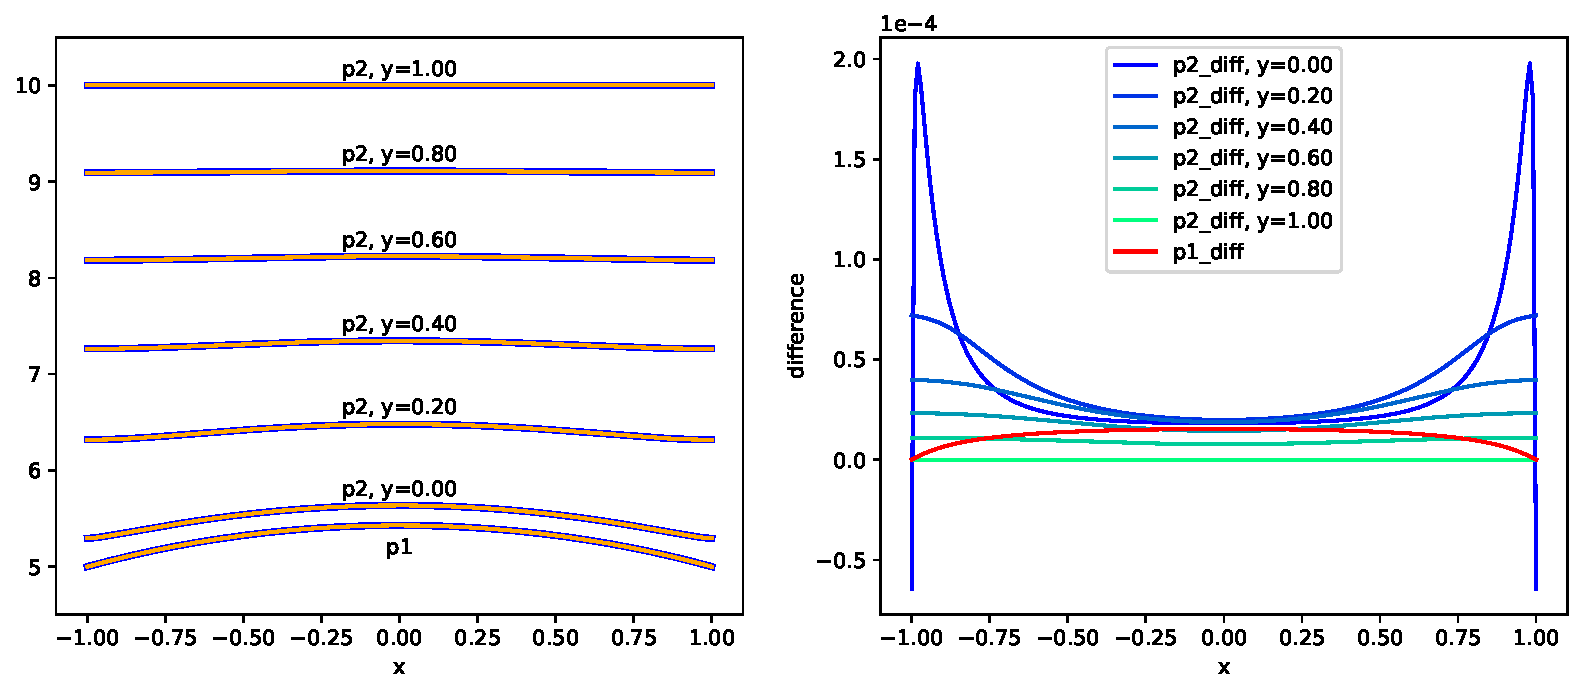
\includegraphics[width=\textwidth]{./continuous_solution.pdf}
  % continuous_convergency.pdf: 0x0 pixel, 300dpi, 0.00x0.00 cm, bb=
  \caption{Conductive fracture case. 
  {\it Left:} Match between the analytical and the numerical solution. 
  {\it Right:} Difference of the analytical and the numerical solution.}
\end{figure}

\begin{figure}
  \label{fig:cont_rate}
  \centering
  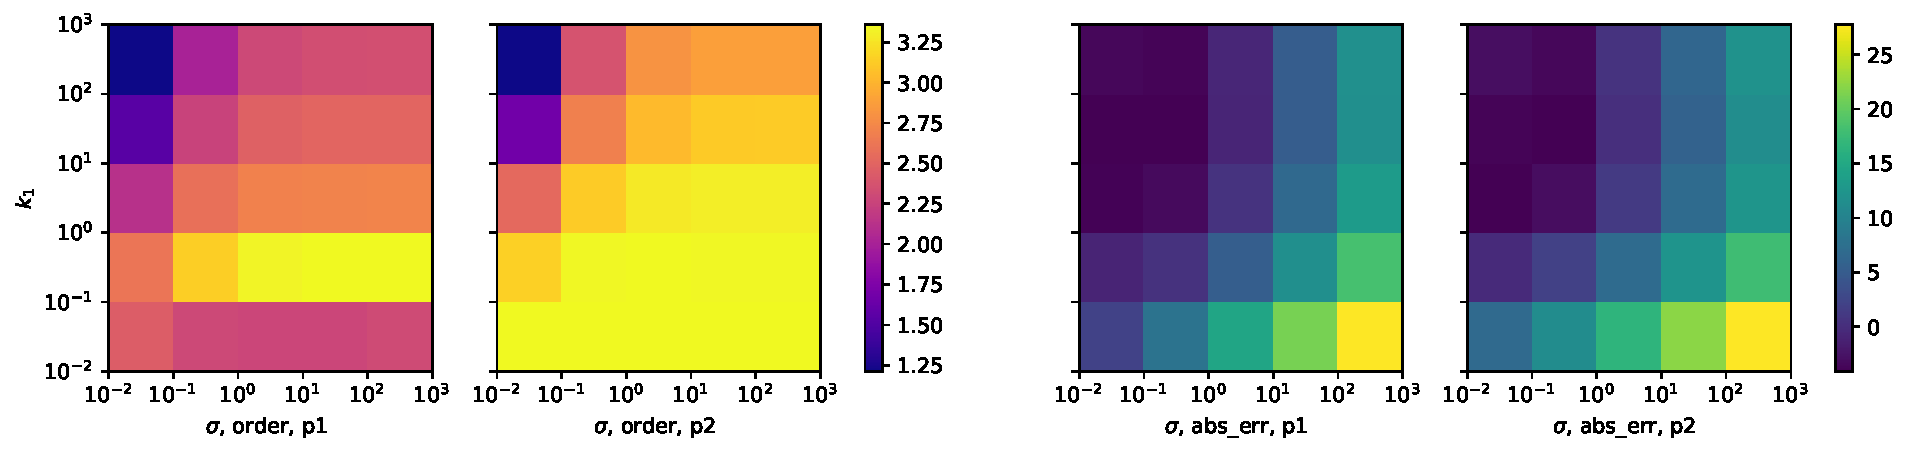
\includegraphics[width=\textwidth]{./continuous_conv_rate.pdf}
  % continuous_convergency.pdf: 0x0 pixel, 300dpi, 0.00x0.00 cm, bb=
  \caption{Convergence rate $p$ and absolute error exponent $c$ as a function of $k_2$ and $\sigma$. 
  {\it Left:} Order of convergence $p$ for $p_1$, $p_2$.
  {\it Right:} Absolute error exponent $c$ for $p_1$, $p_2$.}
\end{figure}





In order to verify correctness of the analytical solution we have implemented a finite difference solution for both the conductive fractue 
and the barrier fracture. We use classical second order differences:
\begin{align*}
    f''(x) &= \frac{-2 f(x) + f(x-h) + f(x+h)}{h^2} + O(h^2),\\
    f'(x) &= \frac{-3 f(x) + 4f(x+h) - f(x+2h)}{2h} + O(h^2)
\end{align*}
wher $h$ is the mesh step.

Figure \ref{fig:cont_solution} presents good match between the numerical solution ($h=0.01$) and the analytical solution (truncation after $1000$ terms). 
Problem parameters were: $\sigma=20$, $k_1=10$, $k_2=1$, $P_2=10$, $P_1=5$.
Estimate for the sum reminder is $10^{-5}$. The magnitude of the error is of order $10^{-4}$. For the whole technically feasible range $h\in (0.1, 0.001)$ 
we have observed perfect second order convergence. 

This is displayed at Figure \ref{fig:cont_rate} which contains results of a parametric study of the 
convergence rate as a function of parameters $k_1 \in [0.01, 0.1, 1, 10, 100]$ and $\sigma$ passing through the same set of values. The pressures $P_2=10$, $P_1=5$
and the conductivity $k_2=1$ are kept constant. For a fixed pair $k_1$, $\sigma$ we have estimated the rate of convergence by computing the finite difference solution for a sequence  
of mesh steps $0.1,\ 0.05,\ 0.025,\ 0.0125$. For every mesh step the $L^2$ errors $\epsilon_1$ and $\epsilon_2$ were approximated by the midpoint rule 
for $p_1$ and $p_2$ respectively. The order of convergence $p$ and the absolute error exponent $c$ were determined by the fit:
\[
        \log_2(\epsilon) \approx -c + p\log_2(h) 
\]

Clearly, the optimal second-order convergence or better is preserved for the majority of the parameter space. The drop to the linear convergence for combination 
of small $k_1$ and large $\sigma$ is due to extreme derivatives of $p_1$ close to the endpoints ${-1, 1}$. This behavior can not be resolved by the used regular grid.
Also, the absolute error exponent is well above $0$ so the error has a small magnitude. 

In the similar fashion we have tested the analytical solution to the barrier case. Shape of the solution and its match with the finite difference approximation 
is shown in Figure \ref{fig:barrier_solution}. The problem parameters were: $k_1=0.5$, $k_2^+=5$, $k_2^-=2$, $\sigma^+=20$, $\sigma^-=10$, $P_1=0$, 
$P_2^+=10$, $P_2^-=-10$, mesh step $h=0.01$. Notice the larger pressure gradient in lower part $\Omega^-$ with smaller conductivity $k_2^- = 2$, also the gap between 
$p_1(x)$ and $p_2(x, 0)$ is larger due to smaller value of $\sigma^- = 10$. 

The convergence rate for varying parameters is shown in Figure \ref{fig:barrier_rate}. In particular we have used $\sigma^+ = 3*\sqrt{\sigma}$, $\sigma^- = \sigma$
and $k_2^+ = k_2$, $k_2^- = \sqrt{k_2}$ with both $\sigma$ and $k_2$ iterating through the list $[0.01, 0.1, 1, 10, 100]$. Remaining parameters were fixed on 
following values: $k_1=1$, $P_2^+=10$, $P_2^-=-10$, $P_1=0$. Overall convergence rate is close to or beyond second order as in the previous case we see problems 
of the finite differences to resolve high gradient in $p_1$ for high $k_2$ and $\sigma$. Absolute error is also small for small $k_2$ which is natural since the 
solution (both $p_1$ and $p_2$) tends to be constant in $x$. 

\begin{figure}
  \label{fig:barrier_solution}
  \centering
  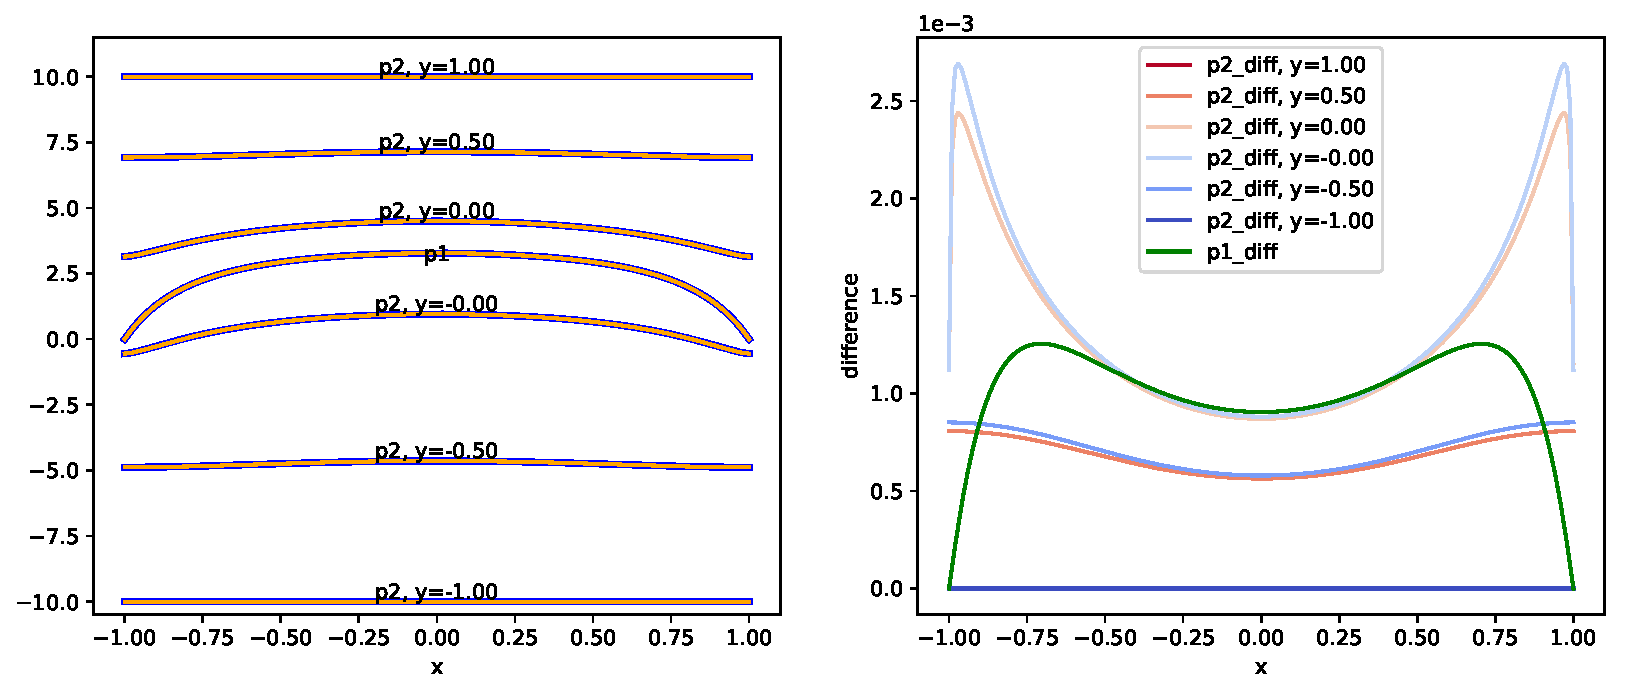
\includegraphics[width=\textwidth, keepaspectratio=true]{./barrier_solution.pdf}
  % continuous_convergency.pdf: 0x0 pixel, 300dpi, 0.00x0.00 cm, bb=
  \caption{Barrier fracture case.
  {\it Left:} Match between the analytical and the numerical solution. 
  {\it Right:} Difference of the analytical and the numerical solution.}
\end{figure}

\begin{figure}
  \label{fig:barrier_rate}
  \centering
  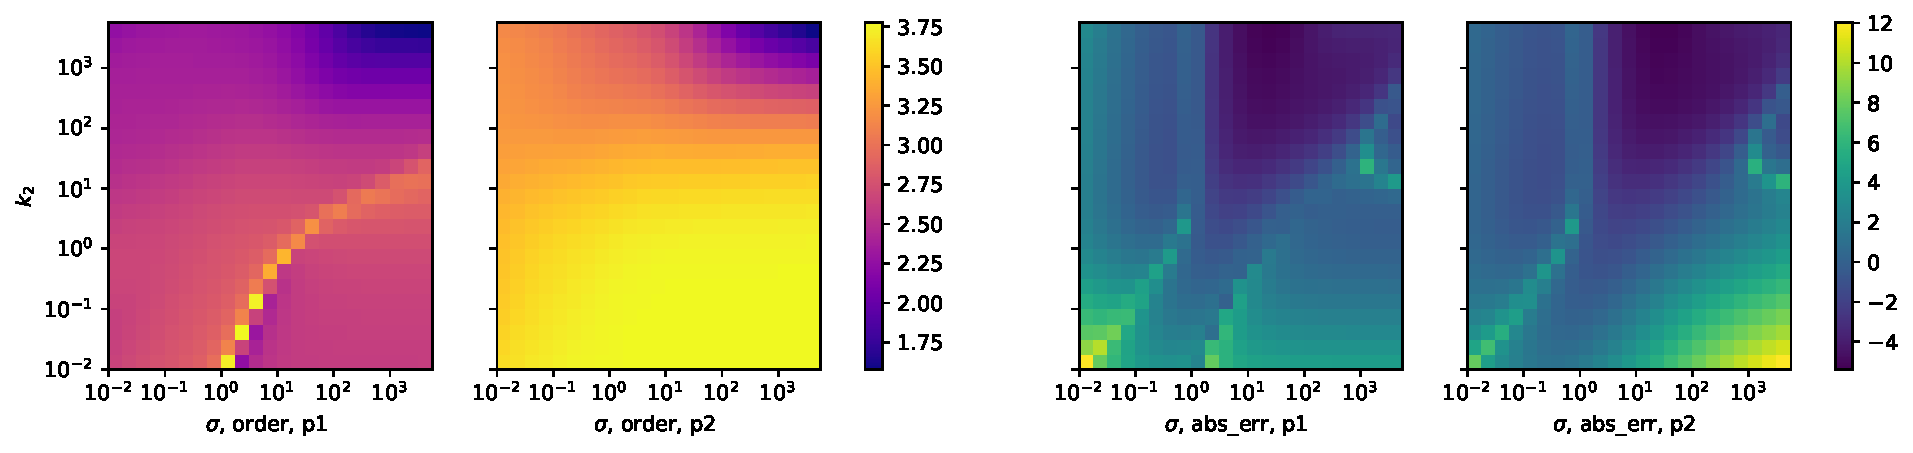
\includegraphics[width=\textwidth]{./barrier_conv_rate.pdf}
  % continuous_convergency.pdf: 0x0 pixel, 300dpi, 0.00x0.00 cm, bb=
  \caption{Convergence rate $p$ and absolute error exponent $c$ as a function of $k_2$ and $\sigma$. 
  {\it Left:} Order of convergence $p$ for $p_1$, $p_2$.
  {\it Right:} Absolute error exponent $c$ for $p_1$, $p_2$.}
\end{figure}


\section{Conclusion}
\label{sec:conclusion}
The analytical solution in a form of Fourier series has been derived for the symmetrical conductive fracture problem as well as for 
the general barrier fracture problem. The solution was modified for practical calculations and the convergence rate of the series was estimated theoretically and 
confirmed numerically. It was realized that summing $100$ terms provides precision about $10^{-6}$ which would be enough for most applications.
The adaptive summation can do even better. The analytical solution was successfully verified against a finite difference solution.  

The analytical solution is used as part of the test suit of the software Flow123d \cite{flow123d} to test various methods of coupling for both conforming 
and non-conforming mixed meshes.



 \bibliographystyle{plain} 
 \bibliography{analytical_fracture.bib}


\end{document}
